\documentclass{article}
\usepackage{pgfplots}
\usepackage{textcomp}
\begin{document}
\begin{figure}


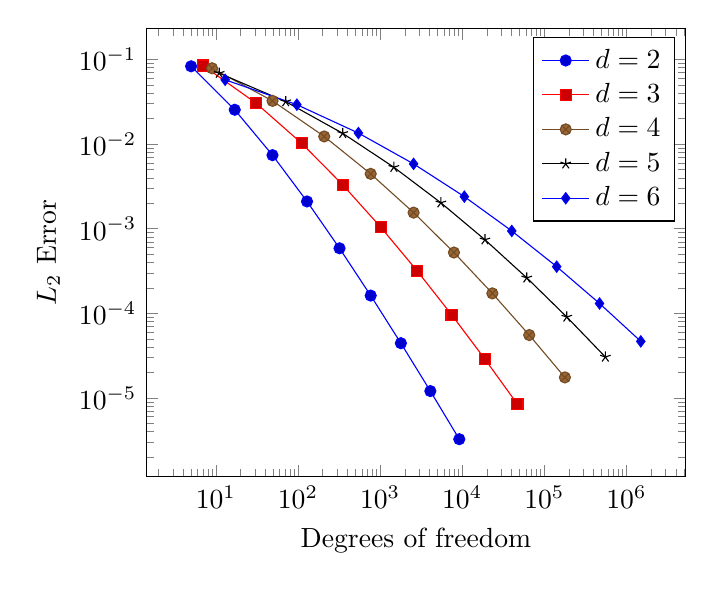
\begin{tikzpicture}
\begin{loglogaxis}[
	xlabel={Degrees of freedom},
	ylabel={$L_2$ Error}
]
\addplot coordinates {
	(5,8.312e-02)    (17,2.547e-02)   (49,7.407e-03)
	(129,2.102e-03)  (321,5.874e-04)  (769,1.623e-04)
	(1793,4.442e-05) (4097,1.207e-05) (9217,3.261e-06)
};

\addplot coordinates{
	(7,8.472e-02)    (31,3.044e-02)    (111,1.022e-02)
	(351,3.303e-03)  (1023,1.039e-03)  (2815,3.196e-04)
	(7423,9.658e-05) (18943,2.873e-05) (47103,8.437e-06)
};

\addplot coordinates{
	(9,7.881e-02)     (49,3.243e-02)    (209,1.232e-02)
	(769,4.454e-03)   (2561,1.551e-03)  (7937,5.236e-04)
	(23297,1.723e-04) (65537,5.545e-05) (178177,1.751e-05)
};

\addplot coordinates{
	(11,6.887e-02)    (71,3.177e-02)     (351,1.341e-02)
	(1471,5.334e-03)  (5503,2.027e-03)   (18943,7.415e-04)
	(61183,2.628e-04) (187903,9.063e-05) (553983,3.053e-05)
};

\addplot coordinates{
	(13,5.755e-02)     (97,2.925e-02)     (545,1.351e-02)
	(2561,5.842e-03)   (10625,2.397e-03)  (40193,9.414e-04)
	(141569,3.564e-04) (471041,1.308e-04) (1496065,4.670e-05)
};
\legend{$d=2$,$d=3$,$d=4$,$d=5$,$d=6$}
\end{loglogaxis}

\end{tikzpicture}

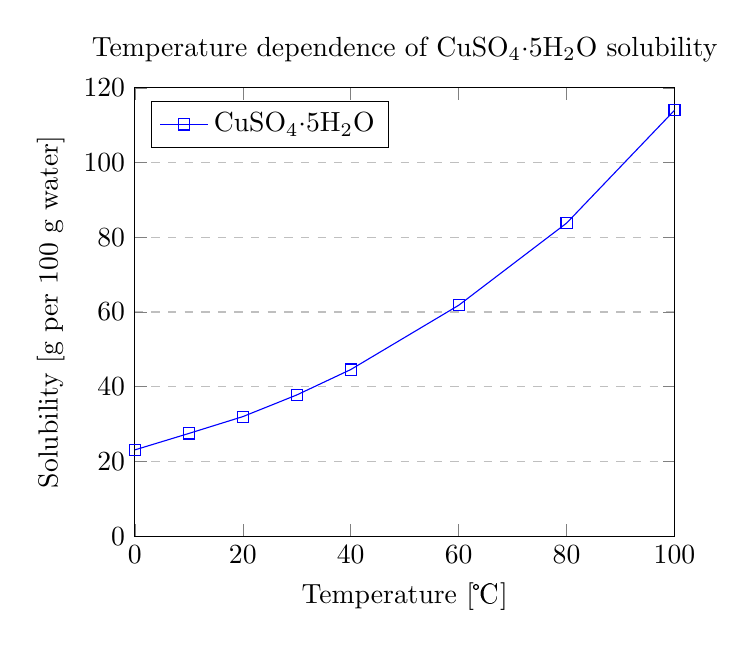
\begin{tikzpicture}
\begin{axis}[
    title={Temperature dependence of CuSO$_4\cdot$5H$_2$O solubility},
    xlabel={Temperature [\textcelsius]},
    ylabel={Solubility [g per 100 g water]},
    xmin=0, xmax=100,
    ymin=0, ymax=120,
    xtick={0,20,40,60,80,100},
    ytick={0,20,40,60,80,100,120},
    legend pos=north west,
    ymajorgrids=true,
    grid style=dashed,
]
 
\addplot[
    color=blue,
    mark=square,
    ]
    coordinates {
    (0,23.1)(10,27.5)(20,32)(30,37.8)(40,44.6)(60,61.8)(80,83.8)(100,114)
    };
    \legend{CuSO$_4\cdot$5H$_2$O}
 
 \end{axis}
\end{tikzpicture}
 \caption{A picture of the same gull           looking the other way!}
\end{figure}
\end{document}
